\documentclass[14pt]{extarticle}

\usepackage[T2A]{fontenc}
\usepackage[utf8]{inputenc}
\usepackage[russian]{babel}

\usepackage[style=numeric,sorting=none]{biblatex}
\addbibresource{coursework.bib}

\usepackage{mathptmx}
\usepackage{gensymb}

\usepackage{amsmath}

\usepackage{geometry}
\geometry{
	a4paper,
	top=20mm,
	bottom=23mm,
	footskip=10mm,
	left=25mm,
	right=15mm
}
\setlength{\parindent}{10mm}
\renewcommand{\baselinestretch}{1.5}

\usepackage{fancyhdr}
\pagestyle{fancy}
\renewcommand{\headrulewidth}{0pt}
\lhead{}
\chead{}
\rhead{}
\lfoot{}
\cfoot{}
\rfoot{\thepage}

\usepackage{indentfirst}

\usepackage{enumitem}

\usepackage{graphicx}
\usepackage[labelformat=simple]{subcaption}
\renewcommand{\thesubfigure}{\textit{\asbuk{subfigure})}}
\usepackage{setspace}
\usepackage[font=small, labelsep=period]{caption}
\captionsetup[figure]{font={small,stretch=1.0}}


%\usepackage[sorting=nty, style=numeric, citestyle=numeric]{biblatex}
%\addbibresource{books}

\usepackage{titlesec}
%\titleformat{\section}[hang]{\Large\bf}{\thesection.}{.5em}{}{}
\titleformat{\section}[hang]{\normalsize\bf}{\thesection.}{.5em}{}{}
%\titleformat{\subsection}[hang]{\large\bf}{\thesubsection.}{.5em}{}{}
\titleformat{\subsection}[hang]{\normalsize\bf}{\thesubsection.}{.5em}{}{}
\titleformat{\subsubsection}[hang]{\normalsize\bf}{\thesubsubsection.}{.5em}{}{}
\titlespacing*{\section}{0mm}{6pt}{6pt}
\titlespacing*{\subsection}{0mm}{6pt}{6pt}
\titlespacing*{\subsubsection}{0mm}{6pt}{6pt}

\usepackage{titletoc}
\titlecontents{section}[3mm]{}{\thecontentslabel.\space\filright}{}{\titlerule*[1pc]{.}\contentspage}
\titlecontents{subsection}[6mm]{}{\thecontentslabel.\space\filright}{}{\titlerule*[1pc]{.}\contentspage}
\titlecontents{subsubsection}[9mm]{}{\thecontentslabel.\space\filright}{}{\titlerule*[1pc]{.}\contentspage}

\usepackage{enumitem}
\setlist{nosep}

\begin{document}
	\setlength{\abovedisplayskip}{6pt}
	\setlength{\belowdisplayskip}{6pt}
	%\setlength{\intextsep}{3pt}
	\setlength{\belowcaptionskip}{-15pt}
	%
	\pagenumbering{arabic}
	\setcounter{page}{3}
	\thispagestyle{fancy}
	%
	\tableofcontents
	%
	\newpage
\section{Введение}
В Институте ядерной физики им. Г. И. Будкера СО РАН проводятся эксперименты на электрон-позитронном коллайдере ВЭПП-2000. Коллайдер имеет два места встречи пучков, в которых установлены детекторы КМД-3 (криогенный магнитный детектор) и СНД (сферический нейтральный детектор). В программу проекта ВЭПП-2000 включено измерение сечений процессов, наблюдаемых при столкновениях электронов и позитронов в диапазоне энергий до 2 ГэВ. В число изучаемых процессов входят процессы с фотонами в конечном состоянии.

Для регистрации фотонов в детекторе КМД-3 используется жидкоксеноновый (LXe) калориметр. Фотон, попадая в калориметр, порождает электромагнитный ливень из вторичных электронов, позитронов и фотонов. Частицы ливня регистрируются сигнальными полосками, расположенными на слоях калориметра. Сработавшие сигнальные полоски группируются в кластеры.

При столкновениях электронов $e^-$ и позитронов $e^+$ большое сечение рождения имеют процессы, содержащие нейтральный пион $\pi^0$ в конечном состоянии. Одним из таких процессов является $e^- e^+ \rightarrow \pi^0 \gamma$. Нейтральный пион с вероятностью 99\% распадается на два фотона $\gamma$. Минимальный угол между фотонами при более высокой энергии пи-мезона становится меньше, и при значении $E_{\pi^0}$ = 1 ГэВ этот угол составляет 0,27 радиана. Электромагнитные ливни таких фотонов в калориметре могут перекрываться, и появляется вероятность принять два слившихся кластера, образованных двумя фотонами, за одиночный кластер от одного фотона. Чтобы увеличить статистику событий, повысить точность измерения сечения и других параметров процесса, необходимо разделять такие кластеры.

Таким образом, требуется разработать алгоритм различения однофотонных и двухфотонных кластеров в LXe калориметре детектора КМД-3. Для решения этой задачи выполнены следующие шаги:
\begin{itemize}
	\item описание детектора КМД-3 и LXe калориметра,
	\item обзор библиотеки TMVA 4 и метода BDT,
	\item анализ задачи разделения кластеров,
	\item обучение алгоритма разделения по методу BDT.
\end{itemize}

Результаты данной работы планируется сравнить с результатами работ [].
\section{Детектор КМД-3 и LXe калориметр}
На рис.~\ref{fig:cmd3} представлена схема криогенного магнитного детектора КМД-3.
\begin{figure}[h!]
	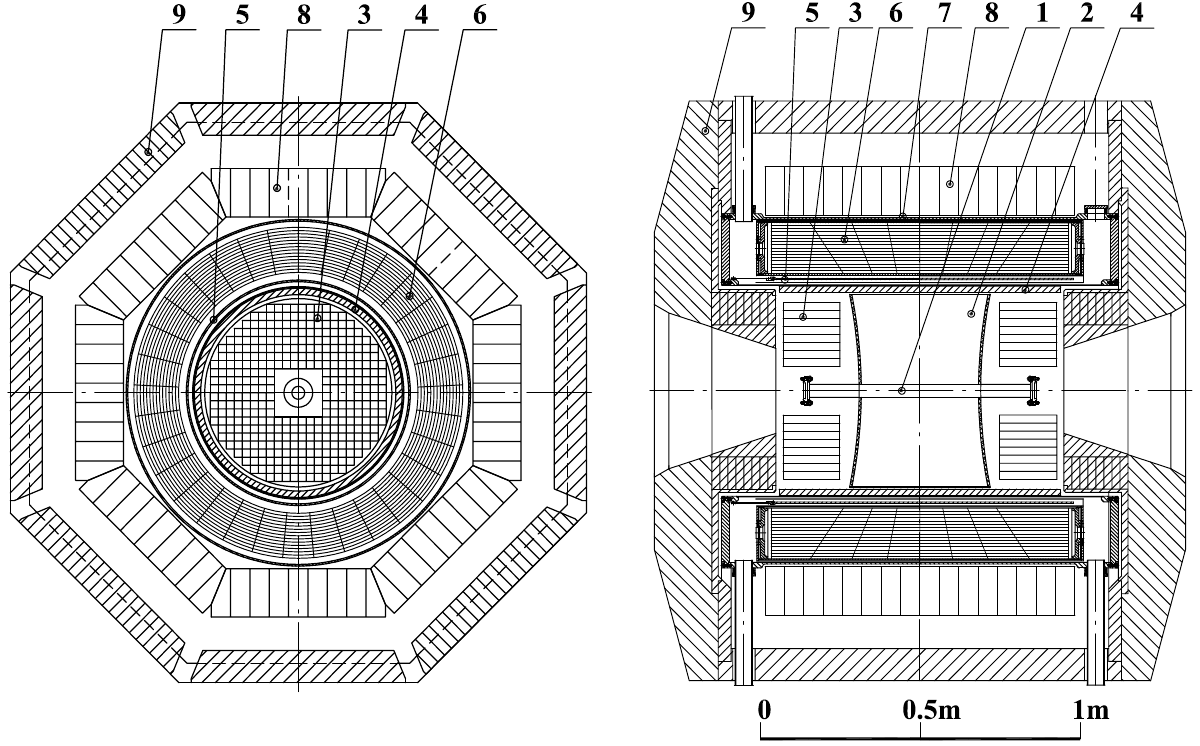
\includegraphics[width=\linewidth]{../pics/cmd3-2.png}
	\caption{Схема детектора КМД-3: 1 -- вакуумная камера, 2 - дрейфовая камера, 3 -- торцевой BGO калориметр, 4 -- Z-камера, 5 -- сверхпроводящий соленоид, 6 -- цилиндрический жидкоксеноновый калориметр, 7 -- времяпролётная система, 8 -- цилиндрический CsI калориметр, 9 -- ярмо магнита}
	\label{fig:cmd3}
\end{figure}

Цилиндрический калориметр детектора регистрирует фотоны и электроны, которые вылетают под большими углами к оси пучков (от $39\degree$ до $141\degree$), и охватывает телесный угол $0,8 \cdot 4\pi$. Он состоит из двух соосных подсистем: жидкоксенонового LXe калориметра и кристаллического CsI калориметра.

Жидкоксеноновый калориметр образован семью соосными катодами и восемью анодами, образующими систему ионизационных камер. Структура электродов LXe калориметра представлена на рис.~\ref{fig:lxe-electrodes}.

\begin{figure}[h!]
	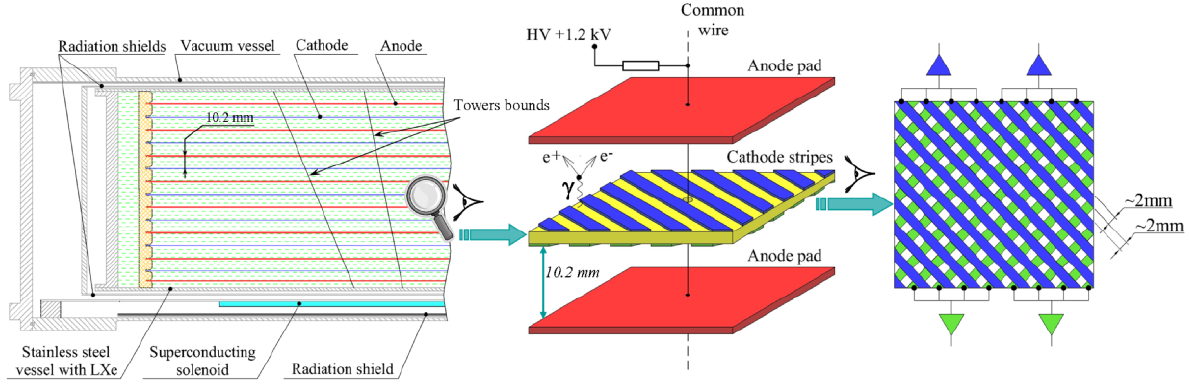
\includegraphics[width=\linewidth]{../pics/lxe-electrodes.png}
	\caption{Структура электродов жидкоксенонового калориметра}
	\label{fig:lxe-electrodes}
\end{figure}

Поверхность каждого анода разделена на 264 прямоугольные площадки -- восемь вдоль оси пучков $Z$, тридцать три в перпендикулярной ей плоскости $R,\varphi$. Площадки с одинаковым положением по $Z$ и $\varphi$ соединены проводником в "башню". Такая "башня" ориентирована в место встречи пучков \cite{shebalin}.
\section{Формат входных данных с калориметра}
\section{Библиотека TMVA и метод BDT}
\section{Алгоритм разделения кластеров}
\section{Результаты}
\section{Заключение}
\section{Список литературы}
\printbibliography
\end{document}